\chapter{动态场景下基于语义信息的位姿估计优化方法}\label{chap:3}
\section{引言}
基于特征的视觉SLAM框架在静态场景下已经具有了较好的鲁棒性和准确度表现,然而在动态场景下的表现却不尽如人意。在场景结构出现变化,如出现走路的人,被抓取移动而的水杯等运动物体时,
场景中静态部分和动态部分在两帧上的投影不满足同一变换关系,因此从图像中静态部分和动态部分提取的特征点不能同时用于两帧间变换矩阵
的计算。换言之,场景中的运动物体为估测相机的运动引入了误差,从而使得SLAM系统整体的状态估计精度降低,甚至会导致跟踪丢失。

针对这一问题,一种直观的解决方案是识别出场景中处于运动状态的物体,将其在二维图像上投影区域内的特征点当做外点移除,从而仅使用
场景中静态部分的特征点进行位姿估计,以提高系统在动态场景下的精确度和鲁棒性。沿袭这一思路,本文提出了一种双阶段的动态外点滤除算法,
此算法结合基于语义类别的自适应权重生成方法和基于极线约束的动态一致性检测方法,能够对于不同类别的物体自适应生成不同的判定条件,
判断其是否处于运动状态,并移除处于运动状态的物体的轮廓内的特征点。本章将就这一方法进行详细介绍,并分析并对比其在公开数据集上的实验结果。

\section{基于极线约束的动态一致性检测方法研究}
\subsection{极线约束}

\begin{figure}[!htbp]
    \centering
    \begin{subfigure}[b]{0.35\textwidth}
      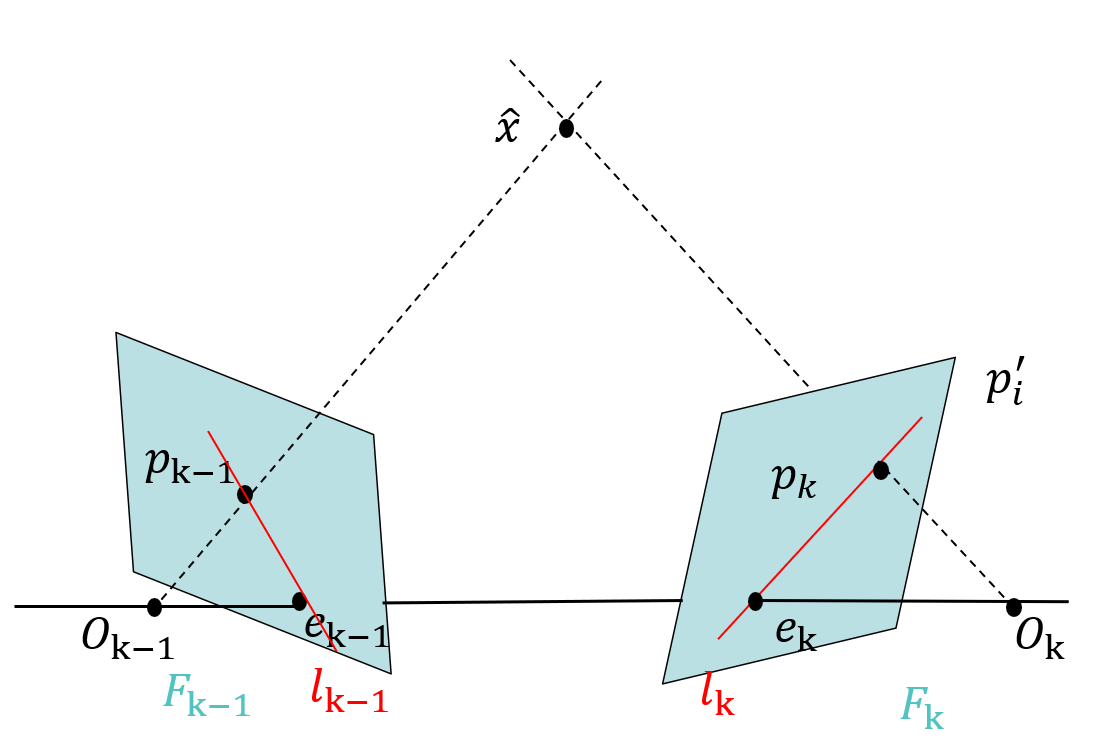
\includegraphics[width=\textwidth]{Img/3-epiplorConstrain.png}
      \caption{}
      \label{fig:epiplorConstrain}
    \end{subfigure}%
    ~% add desired spacing
    \begin{subfigure}[b]{0.35\textwidth}
      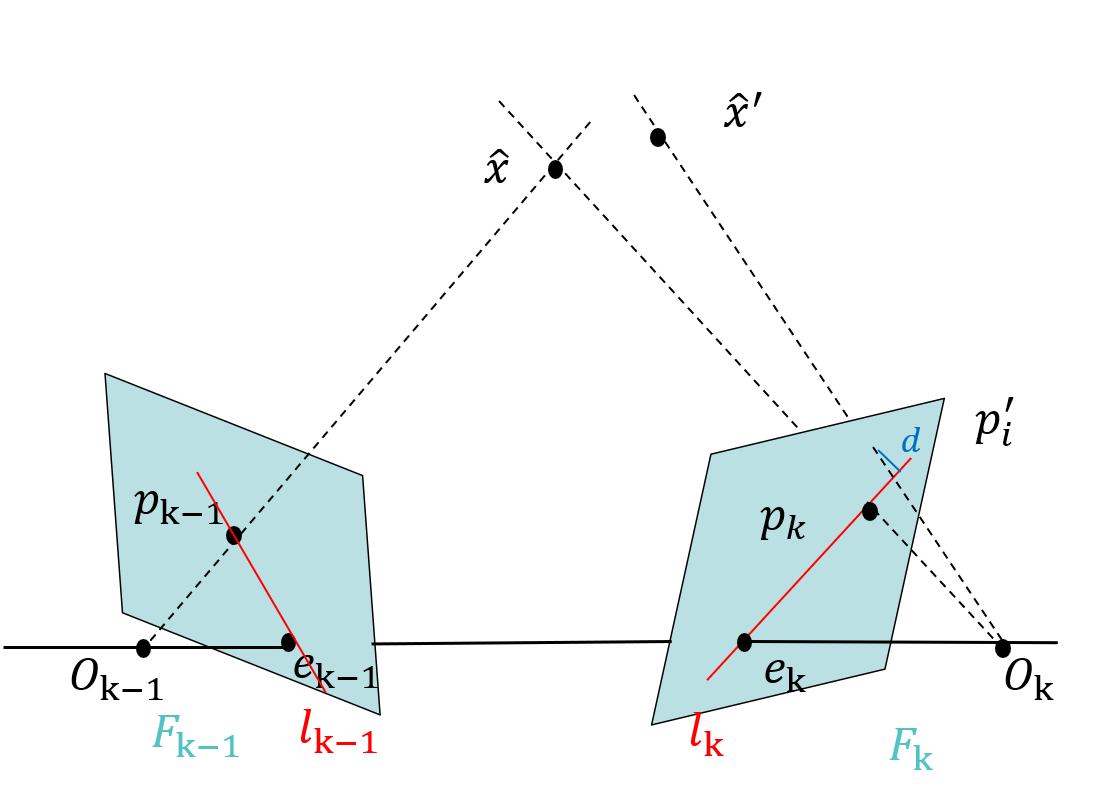
\includegraphics[width=\textwidth]{Img/3-epiplorConstrain2.jpg}
      \caption{}
      \label{fig:epiplorConstrain2}
    \end{subfigure}
    \bicaption{极线约束示意图。(a) 三维点静止时满足极线约束,(b) 三维点运动时不满足极线约束。}{Illustration of epipolar constraint. (a) The epipolar constraint is satisfied when the 3D point is stationary, and (b) the epipolar constraint is not satisfied when the 3D point is in motion.}
    \label{fig:epiplor}
\end{figure}
极线约束如图\ref{fig:epiplor}所示。根据多视图几何原理\citep{hartley2003multiple},对于相机在移动过程中捕捉的连续两帧图像$F_{k-1}$和$F_{k}$,可以提取和匹配
其中一对特征点$P_{k-1}$,$P_{k}$,在静态场景下,$P_{k-1}$和$P_{k}$对应世界坐标系下同一点$\hat{X}=\left[x,y,z\right]^{T}$。
设两帧相机的光心分别为$O_{k-1}$和$O_{k}$,两帧间的运动表示为转移矩阵$T_{k-1,k}=\left[R|t\right]$。两帧相机光心与特征点的连线
$\vec{O_{k-1}P_{k-1}}$、$\vec{O_{k}P_{k}}$会在三维空间中交汇于$\hat{X}=$。

$O_{k-1}$、$O_{k}$、$\hat{X}$三点可以确定一个平面,称作极平面(Epipolar plane),$O_{k-1}$与$O_{k}$两点确定一条直线$O_{k-1}O_{k}$,
称作基线(Baseline),$O_{k-1}O_{k}$与$F_{k-1}$、$F_{k}$分别交于两点$e_{k-1}$、$e_{k}$,称作极点。$e_{k-1}$、$e_{k}$
分别与$P_{k-1}$、$P_{k}$的连线称作极线(Epipolar line),表示为$l_{k-1}$、$l_{k}$,极线也是极平面与$F_{k-1}$和$F_{k}$
的交线。

对于$F_{k-1}$来说,$X$可能位于$\vec{O_{k-1}P_{k-1}}$上任何一点,其在$F_{k-1}$上的投影都是$P_{k-1}$。这些可能的三维点投影在
$F_{k}$上,形成了$\vec{e_{k}P_{k}}$,也就是$F_{k}$的极线$l_{k}$。根据特征点的匹配关系,我们可得而三维点$\hat{X}$在
$F_{k}$上具体的投影位置$P_{k}$,在$\hat{X}$静止不动的前提下,不考虑误差的影响,点$P_{k}$应在极线$l_{k}$上,即极线约束:
$$P_{k}^{T}·l_{k}=0$$
在已知基础矩阵$F$的情况下,根据基础矩阵的定义\citep{hartley2003multiple},有
$$F=e_{k-1}\times H$$
其中$\times$表示叉乘运算,$H$表示$F_{k-1}$与$F_{k}$之间的单应矩阵(Homography),描述了两个平面之间的映射关系。因$e_{k}$
与$P_{k}$同在$l_{k}$上,$l_{k}$又可表示为:
$$l_{k}=e_{k}\times P_{k}$$
因两平面上可以通过单应矩阵变换,可得:
$$P_{k}=HP_{k-1}$$
进而得到:
$$l_{k}=e_{k}\times HP_{k-1}=FP_{k-1}$$
因此极线约束也可写成:
$$P_{k}^{T}·FP_{k-1}=0$$

在静态场景下,同一三维点在两帧上的投影应满足极线约束,$P_{k}$到$l_{k}$的距离$d_{k}$应接近于0。而当三维点处于动态时,如由$\hat{X}$运动至${\hat{X}}^{'}$,极线约束不再满足,
因此,$d_{k}$可以一定程度上反应三维点的运动程度,当$d_{k}$足够大,即有理由认为对应三维点$\hat{X}$处于运动状态。

\subsection{L-K光流法}
由于场景中可能存在处于运动状态物体,通过特征点的匹配集合来计算得出的基础矩阵可能存在误差,因此本算法使用光流法寻找两帧间
像素匹配集合。光流法是基于像素明暗关系对像素的运动进行预测的方法,它能够描述在连续帧间,像素在图像中的运动,通过光流法可预测同一三维点在连续两帧中的位置,获得匹配点坐标。
在本文中,我们选用了经典的L-K光流法(Lucas-Kanade Optical flow)\citep{bouguet2001pyramidal}。

L-K光流法是一种两帧差分的光流估计方法,它假设相机捕获的图像是随时间变化的,对应灰度图$I$是关于时间$t$的函数,可表示为$I_{t}$。
对于三维点$\hat{X}$,在t时刻在图像上的投影可表示为齐次坐标
$$\widetilde{P_{t}}=\left[u,v,1\right]$$
它的灰度值可表示为
$$I(u,v,t)$$
设连续两帧之间该点坐标和时间变化量分别为$du$、$dv$、$dt$,则在经时长为$dt$的变化后,该点可表示为:
$$\widetilde{P_{t+dt}}=\left[u+du,v+dv,1\right]$$
对应的,其灰度值可表示为
$$I(u+du,v+dv,t+dt)$$
光流法的计算基于灰度不变假设,即同一个三维点在不同时刻图像上的投影,其灰度值是保持不变的。据此可以得出:
$$I(u,v,t)=I(u+du,v+dv,t+dt)$$
若两帧间运动量足够小,则可通过泰勒展开进行近似:
$$I(u+du,v+dv,t+dt)\approx I(u,v,t)+\frac{\partial I}{\partial u}du+\frac{\partial I}{\partial v}dy+\frac{\partial I}{\partial t}dt$$
由此得出:
$$\frac{\partial I}{\partial u}du+\frac{\partial I}{\partial v}dy+\frac{\partial I}{\partial t}dt=0$$
进一步变形可得:
$$\frac{\partial I}{\partial u}\frac{du}{dt}+\frac{\partial I}{\partial v}\frac{dv}{dt}=-\frac{\partial I}{\partial t}$$
其中,$\frac{\partial I}{\partial u}$和$\frac{\partial I}{\partial v}$分别为$I(u,v,t)$沿$u$、$v$方向的梯度,$\frac{du}{dt}$
和$\frac{dv}{dt}$分别为像素点$P_{t}$沿$u$、$v$方向运动的速度。将$\frac{\partial I}{\partial u}$和$\frac{\partial I}{\partial v}$
记作$\mathcal{G}=\left[G_{u},G_{v}\right]^{T}$、$\frac{\partial I}{\partial t}dt$记作$G_{t}$、$\frac{du}{dt}$
和$\frac{dv}{dt}$记作$\mathcal{V}=\left[V_{u},V_{v}\right]^{T}$,则上式可以写成:
$$
\mathcal{G}^{T}\cdot \mathcal{V}=
\left[G_{u},G_{v}\right]
\left[
\begin{tabular}{@{}c@{}}
    $V_{u}$ \\ $V_{v}$\\
\end{tabular}
\right]
=
G_{u}V_{u}+ G_{v}V_{v}
=
-G_{t}
$$

发生运动后像素点的坐标值可以通过该像素的运动速度$V_{u}$和$V_{v}$得出,但上式为二元一次方程,无法求出$V_{u}$和$V_{v}$的数值解,
需要引入额外的约束。在L-K光流法中,引入了空间一致性假设,即认为以$P_{t}$为中心,大小为$w\times w$的邻域内,共有$w^{2}$个像素,
所有像素都具有相同的运动速度$\mathcal{V}=\left[V_{u},V_{v}\right]^{T}$,则对于窗口内的所有像素都有:
$$
\begin{array}{l}
    G_{u_{1}}V_{u}+ G_{v_{1}}V_{v}=-G_{t_{1}} \\  
    G_{u_{2}}V_{u}+ G_{v_{2}}V_{v}=-G_{t_{2}} \\ 
    \vdots\\ 
    G_{u_{w^{2}}}V_{u}+ G_{v_{w^{2}}}V_{v}=-G_{t_{w^{2}}} \\  
\end{array}
$$
可以构造超定方程组:
$$
\left[
\begin{array}{l}
    \mathcal{G}_{1}^{T} \\  
    \mathcal{G}_{2}^{T} \\   
    \vdots\\ 
    \mathcal{G}_{w^{2}}^{T} \\   
\end{array}
\right]
\cdot 
\mathcal{V}
=
-
\left[
\begin{array}{l}
    G_{t_{1}}^{T} \\  
    G_{t_{1}}^{T} \\   
    \vdots\\ 
    G_{t_{w^{2}}}^{T} \\   
\end{array}
\right]
$$
记:
$$
\textbf{G}=
\left[
\begin{array}{l}
    \left[G_{u},G_{v}\right]_{1}\\  
    \left[G_{u},G_{v}\right]_{2} \\   
    \vdots\\ 
    \left[G_{u},G_{v}\right]_{w^{2}} \\   
\end{array}
\right]
,
\textbf{b}=
\left[
\begin{array}{l}
    G_{t_{1}}\\  
    G_{t_{2}} \\   
    \vdots\\ 
    G_{t_{w^{2}}} \\   
\end{array}
\right]
$$
可将上述方程组写作:
$$\textbf{G}\cdot\textbf{V}=-\textbf{b}$$
上式可以通过最小二乘法求解,得到像素点$P_{t}$运动速度:
$$
\mathcal{V}=-(\textbf{G}^{T}\textbf{G})^{-1}\textbf{G}^{T}\textbf{b}
$$
根据像素点的运动速度,容易计算出在相机运动后,该像素出现的坐标。在连续两帧$F_{k-1}$、$F_{k}$中,对$F_{k-1}$中的角点使用L-K光流法
跟踪其运动,则可以得到在$F_{k}$上的对应角点集合。因此,可以得到两帧的匹配点集合$\mathbb{P}_{k-1}$、$\mathbb{P}_{k}$。
\subsection{动态一致性检测}
根据上述L-K光流法,可以得出两帧直之间的匹配点集$\mathbb{\widetilde{P}}_{k-1}$、$\mathbb{\widetilde{P}}_{k}$,通过八点法算法,利用匹配点集计算基础矩阵$F$,
具体方法为,对于一对以齐次坐标表示的匹配点$\widetilde{P_{k-1}}=\left[u_{k-1},v_{k-1},1\right]^{T}$和$\widetilde{P_{k}}=\left[u_{k},v_{k},1\right]^{T}$,根据对极几何关系可得:
$$\widetilde{P_{k-1}}^{T}F\widetilde{P_{k}}=0$$
将$F$写成矩阵形式可得:
$$
\left[
\begin{array}{ccc}
    u_{k-1} & v_{k-1} & 1\\
\end{array}
\right]
\left[
\begin{array}{ccc}
    f_{11} & f_{12} & f_{13}\\
    f_{21} & f_{22} & f_{23}\\
    f_{31} & f_{32} & f_{33}\\
\end{array}
\right]
\left[
\begin{array}{l}
    u_{k}\\
    v_{k}\\
    1\\
\end{array}
\right]
=0
$$
将其展开可得到:
$$u_{k}u_{k-1}f_{11}+u_{k}v_{k-1}f_{12}+u_{k}f_{13}+v_{k}u_{k-1}f_{21}+v_{k}v_{k-1}f_{22}+v_{k}f_{23}+u_{k-1}f_{31}+v_{k-1}f_{32}+f_{33}=0$$
将$F$写成向量形式:
$$\mathcal{f}=
\left[
\begin{array}{ccccccccc}
    f_{11} & f_{12} & f_{13} & f_{21} & f_{22} & f_{23} & f_{31} & f_{32} & f_{33}\\
\end{array}
\right]
$$
上式可写成:
$$
\left[
\begin{array}{ccccccccc}
    u_{k}u_{k-1} & u_{k}v_{k-1} & u_{k} & v_{k}u_{k-1} & v_{k}v_{k-1} & v_{k} & u_{k-1} & v_{k-1} & 1\\
\end{array}
\right]
\mathcal{f}
=0
$$
设匹配点集$\mathbb{\widetilde{P}}_{k-1}$、$\mathbb{\widetilde{P}}_{k}$中含有$n$个匹配点对,用其可构造方程组:
$$
\textbf{A}\mathcal{f}=
\left[
\begin{array}{ccccccccc}
    u_{k}^{1}u_{k-1}^{1} & u_{k}^{1}v_{k-1}^{1} & u_{k}^{1} & v_{k}^{1}u_{k-1}^{1} & v_{k}^{1}v_{k-1}^{1} & v_{k}^{1} & u_{k-1}^{1} & v_{k-1}^{1} & 1\\
    \vdots\\
    u_{k}^{n}u_{k-1}^{n} & u_{k}^{n}v_{k-1}^{n} & u_{k}^{n} & v_{k}^{n}u_{k-1}^{n} & v_{k}^{n}v_{k-1}^{n} & v_{k}^{n} & u_{k-1}^{n} & v_{k-1}^{n} & 1\\
\end{array}
\right]
\mathcal{f}
=0
$$
在存在唯一解的情况下,$\textbf{A}$的秩为8,$\mathcal{f}$可以通过最少八组匹配点对解出。由于噪声影响,$\textbf{A}$的秩可能为9,
此时可以求$\mathcal{f}$的最小二乘解,具体方法分求线性解和奇异性约束两步。
\textbf{\emph{求线性解}}

首先对\textbf{A}进行SVD分解求得基本线性解:
$$\textbf{A}=\textbf{U}\textbf{D}\textbf{V}^{T}$$
$\textbf{V}$的最后一列矢量即为$\textbf{A}$最小奇异值对应的奇异向量,也是使得$\|\textbf{A}\mathcal{f}\|$最小的$\mathcal{f}$的解矢量。
\textbf{\emph{奇异性约束}}

得到基本解矢量后,为其增加奇异性约束,确保$F$的奇异性。求最终解为$F^{*}$,满足:
$$
\begin{aligned}{2}
    \min_{F^{*}} \quad & \left \|F-F^{*} \right \| \\
    \mbox{s.t.}\quad & det(F^{*})=0
\end{aligned}
$$
通过SVD分解可求出$F^{*}$,若$F=\textbf{U}\textbf{D}\textbf{V}^{T}$,$\textbf{D}=diag(r,s,t)$,满足$r\geq s \geq t$,
则$F$的最优解为:
$$F^{*}=Udiag(r,s,0)V^{T}$$

为方便描述,之后将八点法求得的基础矩阵最优解$F^{*}$仍记为$F$。求得$F$后,可以计算出像素点$P_{k-1}$对应的极线$l_{k}=\left[x,y,z\right]^{T}$,
进而计算出其匹配点$P_{k}$到$l_{k}$的距离:
$$
d=\frac{\left| P_{k}^{T}FP_{i-1} \right|}{\sqrt{\left \| x^{2}+y^{2}\right \|}}
$$

若$d$超过一定阈值,则认为点$P_{k}$对应的三维点可能处于运动状态,标记$P_{k}$为潜在运动外点。
\section{基于语义类别的自适应权重生成方法研究}
我们注意到,在实际室内场景下,不同种类的物体处于运动状态的可能性也不相同。比如“人”这一类别经常自发行走、活动,很容易处于运动状态;
“椅子”、“水杯”等物体有一定可能性因人为移动等原因而发生移动;而“显示器”,“桌子”等类别的物体,则几乎全程是静止的。因此,
对于不同类别的物体,在相同条件下判断它是否处于运动状态的标准也应有所不同。

本文提出了一种基于先验知识的运动可能性概念,用于自适应地根据目标类别检测结果生成运动状态判定阈值。对于每一类目标,
我们分别为其设置了先验权重$w$,表示这个类别的物体处于运动状态的可能性,数值越大表示这一类别
的物体更倾向于处于静止状态中,特别地,为0表示被预测为此类别的物体不会发生运动,将不参与动态外点的检测过程。
对于当前帧$F_{k}$,在经语义分割模块获取其实例分割结果后,对于检测到的第$j$个目标$r_{j}$,系统将自适应地生成此目标的运动判断阈值:
$$T_{j}=w_{c_{j}}*T_{0}$$
其中$T_{0}$是预设的基础运动判定阈值。$T_{j}$将用于二次判断运动一致性检测阶段得到的潜在运动外点是否处于运动状态,对于位于此
物体区域内的一个像素点$P_{k}$,若其到对应极限的距离满足
$$d>T_{j}$$
则认为此点处于运动状态。

可见,$w$越大类别的物体,在先验假设中认为其更倾向于保持静止,在运动点判定阶段,也自适应地生成了更严苛的判定条件,更不容易
被判断为运动动态。

\section{双阶段的动态外点滤除算法}
\begin{figure}[!htbp]
    \centering
    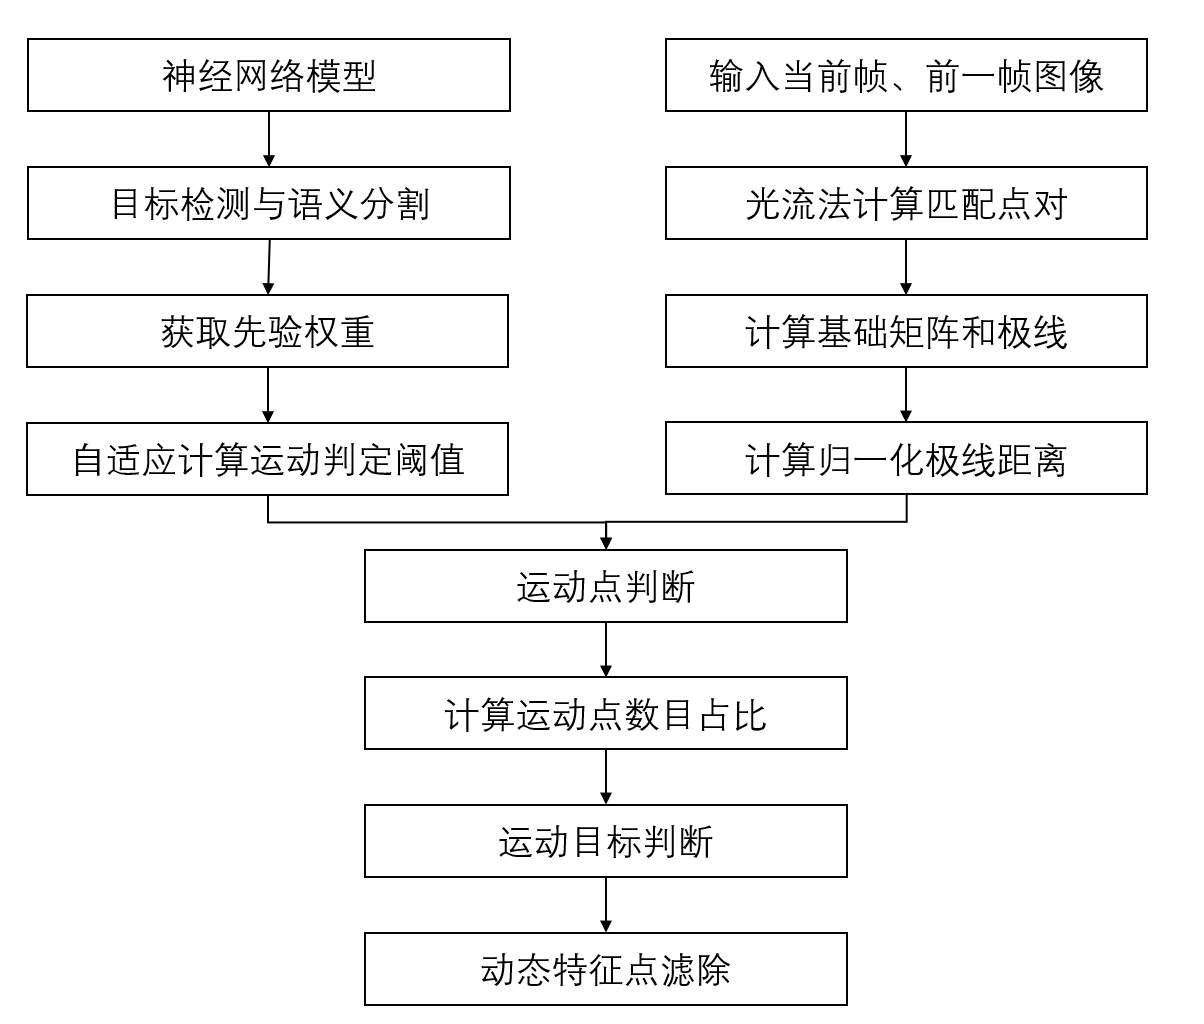
\includegraphics[width=0.6\textwidth]{Img/3-filterflow.png}
    \bicaption{双阶段的动态外点滤除算法流程。}{Workflow of the two-stage dynamic outlier filtering algorithm.}
    \label{fig:filterflow}
\end{figure}
基于以上研究,本文提出了一种双阶段的动态外点滤除算法,结合基于语义类别的自适应权重生成方法和基于极线约束的动态一致性检测方法,
自适应调整不同类别物体的动态点判断阈值,让运动目标检测过程更加平滑,同时结合语义分割结果,能够更精确地仅滤除运动目标范围内的特征点,算法流程如图\ref{fig:filterflow}所示。

在第一阶段,结合语义分割模块预测得到的实例分割结果,系统将通过自适应权重生成方法为其生成运动判断阈值。在第二阶段,将采用运动一致性
检测算法,首先通过L-K光流得到匹配点集并计算得出基础矩阵,并筛选出运动外点。对于每一个检测到的目标$r_{j}$,其位置框$b_{j}$为矩形区域,
对于匹配点集中的点$P_{k}=(u,v)$,若满足:
\begin{equation} 
    \adddotsbeforeeqnnum%
    \begin{cases}
        bu_{j}\geq u\geq bu_{j}+bw_{j}\\
        bv_{j}\geq v\geq bv_{j}+bh_{j}\\
        m(u,v)=c_{j}\\ 
    \end{cases}
\end{equation}
则认为$P_{k}$是此物体的一个前景点,而若$P_{k}$同时满足$d_{k}>T_{j}$,则认为此点是一运动点。统计一个目标所含前景点和运动点的数目,
表示为$N_{object}$和$N_{moving}$,计算运动点占前景点的比例:
$$\eta_{moving}=\frac{N_{moving}}{N_{object}}$$
若$\eta_{moving}$大于一个预设比例阈值$\xi$,我们认为物体$r_{j}$处于运动状态,继而将所有属于其前景部分的特征点移除,以此确保
最大程度上减小环境中动态物体的影响,并减少非目标前景的静态点的误移除。

此算法具体描述为:
\begin{algorithm} %算法开始 
    \small
    \caption{动态外点滤除算法} \label{alg1} %算法的标签 
    \begin{algorithmic}[1] %此处的[1]控制一下算法中的每句前面都有标号 
    \Procedure{滤除后的特征点集合}$\mathbb{f}_{k}$
    %\REQUIRE 当前帧, $F_{k}$;上一帧, $F_{k-1}$;物体检测结果集合$\mathbb{R}$;基础运动判定阈值$T_{0}$
    %\ENSURE 滤除后的特征点集合,$\mathbb{f}_{k}$;
    % if-then-else 
    \State ${\mathbb{f}}_{k}^{'}=ExtractORBKeyPoints(F_{k})$
    \State $p_{k},p_{k-1}=CalOpticalFlowM atching(F_{k-1},F_{k})$
    \State $F=FindFundamentalMat(p_{k-1},p_{k})$
    \For{each $r_{j}$ in $\mathbb{R}$}
    \State $T_{j}=CalMotionT resh(w_{c_{j}},T_{0})$
    \For{each $p_{k}^{i}$ in $r_{j}$}
    \If{$IsForeground(p_{k}^{i},b_{j},m)$}
    \State $l^{i}=CalEpipolarLine(F,p_{k-1}^{i})$
    \State $d^{i}=CalDistoEpipolarLine(l^{i},p_{k}^{i})$
    \If{$d_{k}$ bigger than $T_{k}$}
    \State $N_{moving}\gets N_{moving}+1$
    \EndIf
    \State $N_{object}\gets N_{object}$
    \EndIf
    \EndFor
    \State $\eta_{moving}=CalMovingRatio(N_{moving},N_{object})$
    \If{$\eta_{moving}$大于$\xi$}
    \For{each $f_{i}^{k}$ in $F_{i}^{'}$}
    \If{$IsForeground(f_{i}^{k},b_{j},m)$}
    \State $F_{i}=RemoveOutliers(F_{i}^{'},f_{i}^{k})$
    \EndIf
    \EndFor
    \EndIf
    \EndFor
    \EndProcedure
    \end{algorithmic} 
\end{algorithm}


\section{实验结果与分析}
\subsection{轨迹误差评测}
我们使用TUM RGB-D数据集\citep{sturm2012benchmark}测试了双阶段的动态外点滤除算法在动态环境下对相机位姿估计的优化效果。
TUM RGB-D数据集是由德国慕尼黑工业大学计算机视觉实验室于2012年发布的RGB-D数据集,在当前有着广泛的应用,它使用Microsoft Kinect
以视频帧率(30 Hz)记录,共包含39个序列,每个序列都包含全传感器分辨率(640x 480)下的彩色和深度图像,主要针对纹理丰富的室内办公室场景。

我们选取了了两个场景的片段:
{
\setlist[enumerate]{}% restore default behavior
\begin{enumerate}[nosep]
    \item 走动场景\\高度动态性的以办公区域为主场景,两个人在桌子前后站起、来回走动、坐下。
    \item 对坐场景\\较低动态性以办公区域为主场景,两个人坐在桌子前交谈,辅以手势进行交流,时而小幅度运动。
\end{enumerate}
}

这两个场景都分别使用了四种相机运动方式来记录,包括:
{
\setlist[enumerate]{}% restore default behavior
\begin{enumerate}[nosep]
    \item halfsphere方式\\相机跟随直径为一米的半球的轨迹移动来记录。
    \item xyz方式\\相机沿x、y、z轴移动来记录。
    \item rpy方式\\相机在俯仰角、偏航角、翻滚角上旋转来记录。
    \item static方式\\相机手动保持静态来记录。
\end{enumerate}
}

通过以上四种记录方式记录两个场景,共构成八个序列片段,分别命名为\emph{sitting\_halfsphere}、\emph{sitting\_rpy}、\emph{sitting\_xyz}、\emph{sitting\_static}、\emph{walking\_halfsphere}、\emph{walking\_rpy}、\emph{walking\_xyz}、\emph{walking\_static}其中一些序列是高度动态的,这对于传统的基于特征的视觉SLAM系统来说很难处理。
我们使用这八个片段,测试了本文所提出的位姿估计优化方法,并与此方法的基础SLAM框架ORB-SLAM2实验数据进行了对比,对于每个片段
我们都运行了五次,并对结果取平均值。在我们的实验中,
我们设置“人”这一类别的先验权重为1,“椅子”这一类别的先验权重为5,其余如“键盘”、“显示器”等类别为0。

在实验数据的评估方面,我们使用了绝对轨迹误差(Absolute Trajectory Error,ATE)和相对位姿误差(d Relative Pose Error,RPE)作为评价标准,
其中,绝对轨迹误差能够评估相机轨迹的全局一致性,而相对位姿误差可以评估相机位姿在平移和旋转两方面的误差漂移。我们对整个轨迹
按固定步长采样,计算每个采样点的误差,并以四种方式计算得出全局误差:
{
\setlist[enumerate]{}% restore default behavior
\begin{enumerate}[nosep]
    \item 均方根误差(Root Mean Square Error,RMSE)\citep{pathak2016context}\\表示所有误差项的均方根。
    \item 均值\\表示估计所有误差项的均值。
    \item 中位数\\表示所有误差项的中位数。
    \item 标准差(Standard Deviation,S.D.)\\表示所有误差项的标准差。
\end{enumerate}
}
\begin{table*}[!htbp]
    \bicaption{绝对轨迹误差对比结果。}{RESULTS OF METRICS ABSOLUTE TRAJECTORY ERROR (ATE).}
    \label{tab:ATE}
    \centering
    \footnotesize% fontsize
    \setlength{\tabcolsep}{8pt}% column separation
    \renewcommand{\arraystretch}{1.3}%row space 
    \begin{tabular}{l|cccc|cccc}
        \hline
        & \multicolumn{4}{c|}{ORB SLAM2}                                         & \multicolumn{4}{c}{本文所提出的系统}                                        \\ \hline
        & RMSE            & median          & mean            & std             & RMSE            & median          & mean            & std             \\ \hline
        sitting\_halfsphere & 0.0198          & 0.0127          & 0.0151          & 0.0127          & \textbf{0.0156} & \textbf{0.0122} & \textbf{0.0137} & \textbf{0.0073} \\ \hline 
        sitting\_rpy        & \textbf{0.0197} & \textbf{0.0120} & \textbf{0.0157} & \textbf{0.0120} & 0.0201          & 0.0123          & 0.0158          & 0.0121          \\ \hline
        sitting\_static     & 0.0085          & 0.0071          & 0.0076          & 0.0038          & \textbf{0.0063} & \textbf{0.0048} & \textbf{0.0055} & \textbf{0.0032} \\ \hline
        sitting\_xyz        & \textbf{0.0090} & \textbf{0.0073} & \textbf{0.0079} & \textbf{0.0045} & 0.0101          & 0.0083          & 0.0090          & 0.0046          \\ \hline
        walking\_halfsphere & 0.7057          & 0.5928          & 0.6113          & 0.3527          & \textbf{0.0360} & \textbf{0.0244} & \textbf{0.0300} & \textbf{0.0200} \\ \hline
        walking\_rpy        & 0.8111          & 0.6513          & 0.7091          & 0.3939          & \textbf{0.1448} & \textbf{0.0789} & \textbf{0.1071} & \textbf{0.0773} \\ \hline
        walking\_static     & 0.4237          & 0.3247          & 0.3864          & 0.1739          & \textbf{0.0090} & \textbf{0.0073} & \textbf{0.0081} & \textbf{0.0039} \\ \hline
        walking\_xyz        & 0.7287          & 0.5802          & 0.6463          & 0.3366          & \textbf{0.0197} & \textbf{0.0127} & \textbf{0.0154} & \textbf{0.0112} \\ \hline
        \hline
    \end{tabular}
\end{table*}

\begin{table*}[!htbp]
    \bicaption{相对位姿误差旋转项对比结果。}{RESULTS OF METRIC ROTATIONAL DRIFT (RPE).}
    \label{tab:RPER}
    \centering
    \footnotesize% fontsize
    \setlength{\tabcolsep}{8pt}% column separation
    \renewcommand{\arraystretch}{1.3}%row space 
    \begin{tabular}{l|cccc|cccc}
        \hline
        & \multicolumn{4}{c|}{ORB SLAM2}                                         & \multicolumn{4}{c}{本文所提出的系统}                                        \\ \hline
        & RMSE            & median          & mean            & std             & RMSE            & median          & mean            & std             \\ \hline
        sitting\_halfsphere & \textbf{0.5822} & \textbf{0.4613} & \textbf{0.5119} & \textbf{0.2774} & 0.6497          & 0.5123          & 0.5735          & 0.3052          \\ \hline
        sitting\_rpy        & \textbf{0.7889} & \textbf{0.5852} & \textbf{0.6771} & \textbf{0.4048} & 0.8170          & 0.5939          & 0.6981          & 0.4146          \\ \hline
        sitting\_static     & 0.2878          & 0.2504          & 0.2595          & 0.1244          & \textbf{0.2722} & \textbf{0.2311} & \textbf{0.2437} & \textbf{0.1201} \\ \hline
        sitting\_xyz        & \textbf{0.4701} & \textbf{0.3429} & \textbf{0.3988} & \textbf{0.2490} & 0.4850          & 0.3518          & 0.4115          & 0.2561          \\ \hline
        walking\_halfsphere & 9.5391          & 2.3127          & 6.3003          & 7.1624          & \textbf{0.8587} & \textbf{0.6772} & \textbf{0.7504} & \textbf{0.4160} \\ \hline
        walking\_rpy        & 9.0072          & 2.9693          & 6.1350          & 6.5948          & \textbf{2.4676} & \textbf{0.9672} & \textbf{1.6239} & \textbf{1.8056} \\ \hline
        walking\_static     & 4.2935          & 0.3997          & 1.8289          & 3.8844          & \textbf{0.2745} & \textbf{0.2341} & \textbf{0.2481} & \textbf{0.1167} \\ \hline
        walking\_xyz        & 6.9545          & 2.4975          & 4.7607          & 5.0696          & \textbf{0.6555} & \textbf{0.4329} & \textbf{0.5221} & \textbf{0.3880} \\ \hline
        \hline
    \end{tabular}
\end{table*}
\begin{table*}[!htbp]
    \bicaption{相对位姿误差平移项对比结果。}{RESULTS OF METRIC TRANSLATIONAL DRIFT (RPE).}
    \label{tab:RPET}
    \centering
    \footnotesize% fontsize
    \setlength{\tabcolsep}{8pt}% column separation
    \renewcommand{\arraystretch}{1.3}%row space 
    \begin{tabular}{l|cccc|cccc}
        \hline
        & \multicolumn{4}{c|}{ORB SLAM2}                                         & \multicolumn{4}{c}{本文所提出的系统}                                        \\ \hline
        & RMSE            & median          & mean            & std             & RMSE            & median          & mean            & std             \\ \hline
        sitting\_halfsphere & 0.0227          & 0.0119          & 0.0162          & 0.0159          & \textbf{0.0190} & \textbf{0.0152} & \textbf{0.0168} & \textbf{0.0088} \\ \hline
        sitting\_rpy        & \textbf{0.0248} & \textbf{0.0160} & \textbf{0.0203} & \textbf{0.0143} & 0.0261          & 0.0170          & 0.0214          & 0.0147          \\ \hline
        sitting\_static     & 0.0095          & 0.0075          & 0.0084          & 0.0046          & \textbf{0.0078} & \textbf{0.0060} & \textbf{0.0068} & \textbf{0.0038} \\ \hline
        sitting\_xyz        & \textbf{0.0115} & \textbf{0.0090} & \textbf{0.0100} & \textbf{0.0058} & 0.0125          & 0.0098          & 0.0109          & 0.0060          \\ \hline
        walking\_halfsphere & 0.4451          & 0.0883          & 0.2889          & 0.3386          & \textbf{0.0369} & \textbf{0.0261} & \textbf{0.0306} & \textbf{0.0205} \\ \hline
        walking\_rpy        & 0.4581          & 0.1554          & 0.3105          & 0.3369          & \textbf{0.1230} & \textbf{0.0453} & \textbf{0.0795} & \textbf{0.0921} \\ \hline
        walking\_static     & 0.2388          & 0.0185          & 0.1003          & 0.2167          & \textbf{0.0105} & \textbf{0.0084} & \textbf{0.0094} & \textbf{0.0047} \\ \hline
        walking\_xyz        & 0.3682          & 0.1400          & 0.2514          & 0.2690          & \textbf{0.0245} & \textbf{0.0160} & \textbf{0.0196} & \textbf{0.0136} \\ \hline
        \hline
    \end{tabular}
\end{table*}

测量数据如表\ref{tab:ATE}-表\ref{tab:RPET}所示,可以看出,本文所提出的SLAM系统在走动场景中,相比ORB-SLAM2,无论在绝对轨迹误差还是相对位姿误差
上都取得了量级式的误差降低,这说明了在高度动态的环境下,本文所提出的方法能够显著提升系统的位姿估计精度和鲁棒性。然而,在较低
动态性的对坐场景中,本文所提出的SLAM系统相比于ORB-SLAM2的取得了略微的提升,或二者的数值差异不大,经分析,我们认为导致在轻度动态
场景下提升不够明显这一现象的原因是,动态外点滤除算法减少了用于位姿估计的ORB特征点总数,使得迭代优化过程中没有足够的约束支撑。
另一个不可忽视的原因是,ORB-SLAM2作为当前表现优异的SLAM系统之一,其在静态场景下已经取得了足够高的精度,因此提升空间是十分有限的。

图\ref{fig:trajectory}展示了对于片段\emph{walking\_xyz},ORB-SLAM2和本文所提出的系统的预测以及真值的轨迹可视化对比。

\begin{figure*}[h]
    \centering
    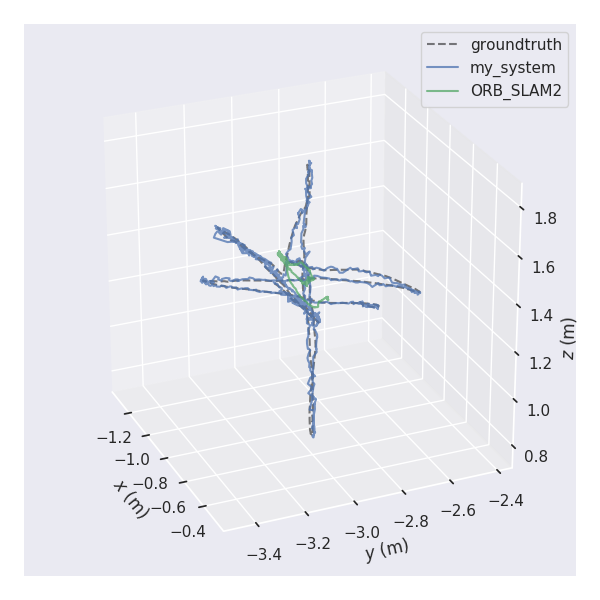
\includegraphics[width=0.31\textwidth]{Img/evo1.png}
    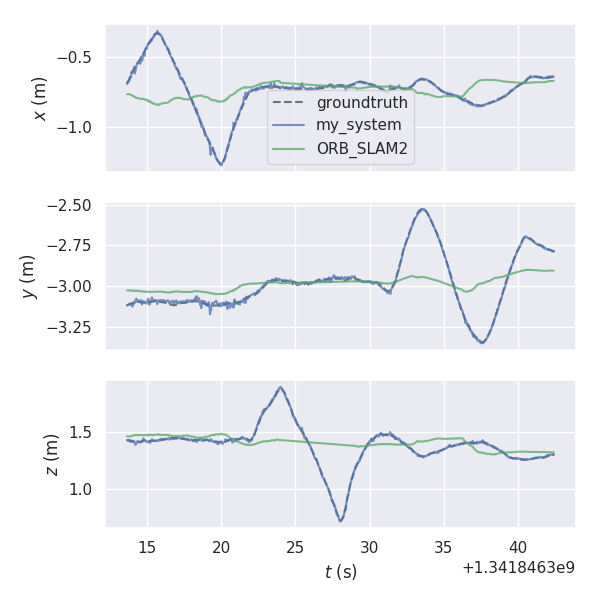
\includegraphics[width=0.31\textwidth]{Img/evo2.png}
    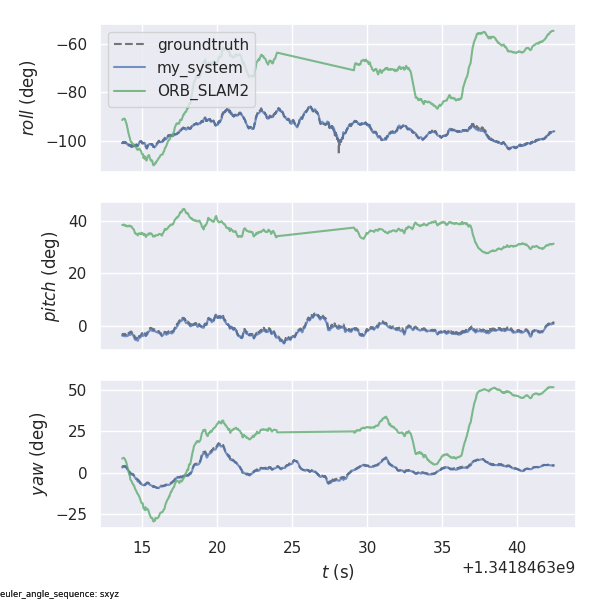
\includegraphics[width=0.31\textwidth]{Img/evo3.png}
    \caption{对于片段\emph{walking\_xyz},ORB-SLAM2和本文所提出的系统的预测以及真值的轨迹可视化对比。}
    \label{fig:trajectory}
  \end{figure*}

本文所提出的SLAM系统也与当前表现最优异的面向动态环境的语义SLAM系统进行了对比,包括DS-SLAM和DynaSLAM。为了避免不同运行环境
引入的实验数据误差,本文直接引用了对比系统原始论文中发布的改进方法和基础方法的测试数据,DS-SLAM、DynaSLAM和本文所提出的方法
都以ORB-SLAM2为基础方法,因此,我们计算了各自改进相对于ORB-SLAM2的提升幅度以进行比较。具体计算方法如下:
$$\rho=\frac{e_{0}-e}{e_{0}}*100$$
其中,$e_{0}$为ORB-SLAM2的误差值,$e$为改进方法的误差值,$\rho$表示误差减少的百分比。
\begin{table*}[!htbp]
    \bicaption{与DS-SLAM的对比结果\citep{YuDS}。}{Comparison of DS-SLAM\citep{YuDS}.}
    \label{tab:DSSLAM}
    \centering
    \footnotesize% fontsize
    \setlength{\tabcolsep}{8pt}% column separation
    \renewcommand{\arraystretch}{1.3}%row space 
    \begin{tabular}{l|ccc|ccc}
        \hline
        & \multicolumn{3}{c|}{DS-SLAM}                                       & \multicolumn{3}{c}{本文所提出的系统}                                    \\ \hline
        & RPET & RPER & ATE            & RPET         & RPER         & ATE            \\ \hline
sitting\_static     & 17.61                    & 5.07                  & \textbf{25.94} & \textbf{18.39}           & \textbf{5.41}         & 25.45          \\ \hline
walking\_halfshpere & 91.62                    & 88.96                 & 93.76          & \textbf{91.70}           & \textbf{91.00}        & \textbf{94.89} \\ \hline
walking\_rpy        & 64.64                    & 62.82                 & 48.97          & \textbf{73.14}           & \textbf{72.60}        & \textbf{82.15} \\ \hline
walking\_static     & 95.27                    & 93.09                 & 97.91          & \textbf{95.59}           & \textbf{93.61}        & \textbf{97.88} \\ \hline
walking\_xyz        & 91.93                    & 89.32                 & 96.71          & \textbf{93.35}           & \textbf{90.57}        & \textbf{97.30} \\ \hline
        \hline
    \end{tabular}
\end{table*}

\begin{table*}[!htbp]
    \bicaption{与DynaSLAM的对比结果\citep{BertaDynaSLAM}。}{Comparison of DynaSLAM\citep{BertaDynaSLAM}.}
    \label{tab:DynaSLAM}
    \centering
    \footnotesize% fontsize
    \setlength{\tabcolsep}{8pt}% column separation
    \renewcommand{\arraystretch}{1.3}%row space 
    \begin{tabular}{l|c|c}
        \hline
        & \multicolumn{1}{c|}{DynaSLAM}         & \multicolumn{1}{c}{本文所提出的系统}           \\ \hline
      %  & DynaSLAM          & our system        \\ \hline
        sitting\_halfsphere & 15                & \textbf{21.0869}  \\ \hline
        sitting\_xyz        & -66.6667          & \textbf{-12.7556} \\ \hline
        walking\_halfsphere & 92.87749          & \textbf{94.8932}  \\ \hline
        walking\_rpy        & \textbf{94.71299} & 82.1502           \\ \hline
        walking\_static     & 93.33333          & \textbf{97.8809}  \\ \hline
        walking\_xyz        & 96.73203          & \textbf{97.2958}  \\ \hline
        \hline
    \end{tabular}
\end{table*}
表\ref{tab:DSSLAM}展示了与DS-SLAM在绝对轨迹误差、相对位姿误差上比较结果,误差项使用RMSE计算,其中RPET和RPER分别代表相对位姿误差
的平移和旋转误差偏移。表\ref{tab:DynaSLAM}展示了与DynaSLAM在绝对轨迹误差项上的提升对比,误差项使用RMSE计算。
这些数据证明了本文所提出的优化方法在几乎所有项上都取得了比当前最优秀的SLAM方法更多的提升,这从侧面证明了本文所提出的有效性。

\subsection{特征点滤除效果评测}
\begin{figure}[!htbp]
    \centering
    \begin{subfigure}[b]{0.35\textwidth}
      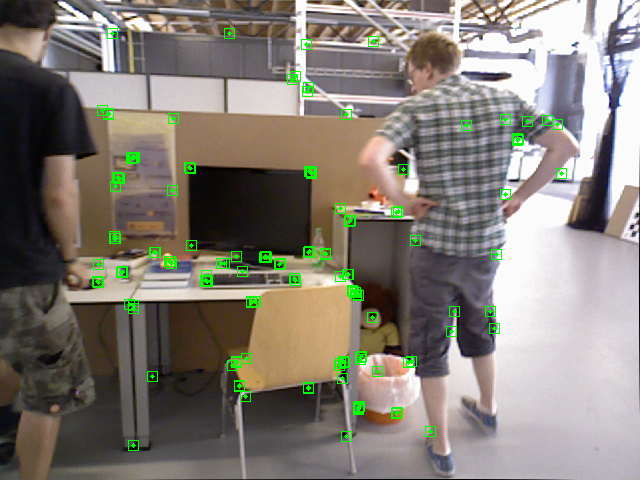
\includegraphics[width=\textwidth]{Img/orb_63.png}
      \caption{}
      \label{fig:orb_63}
    \end{subfigure}%
    ~% add desired spacing
    \begin{subfigure}[b]{0.35\textwidth}
      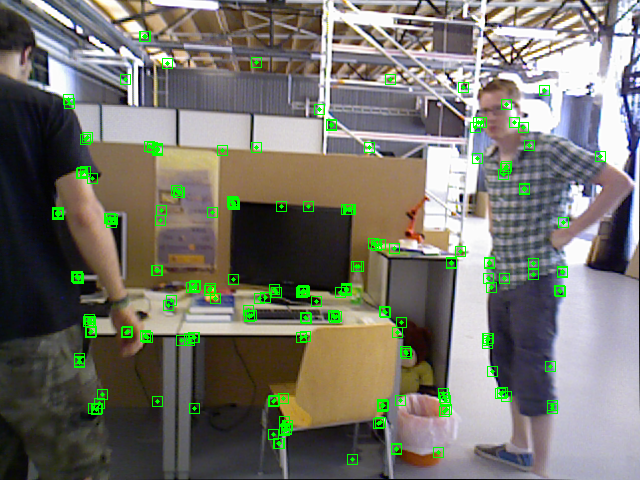
\includegraphics[width=\textwidth]{Img/orb_87.png}
      \caption{}
      \label{fig:orb_87}
    \end{subfigure}
    \\% line break
    \begin{subfigure}[b]{0.35\textwidth}
      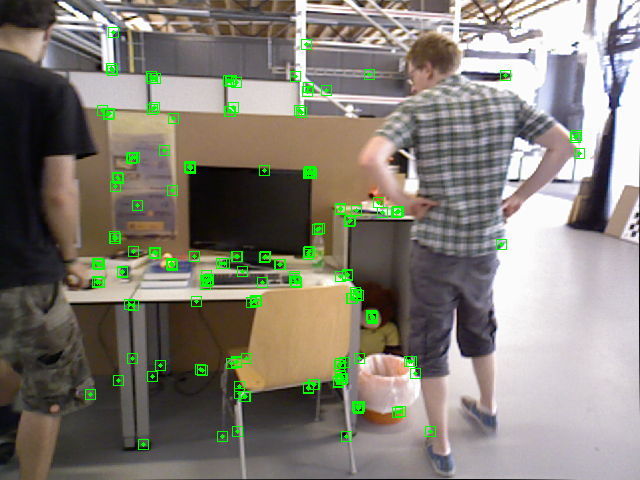
\includegraphics[width=\textwidth]{Img/filter_63.png}
      \caption{}
      \label{fig:filter_63}
    \end{subfigure}%
    ~% add desired spacing
    \begin{subfigure}[b]{0.35\textwidth}
      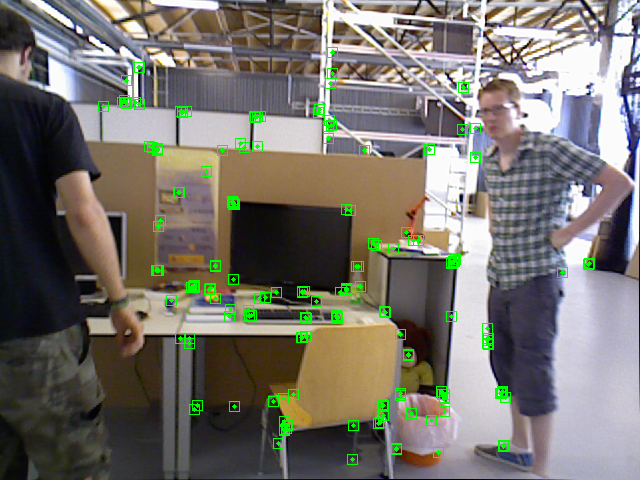
\includegraphics[width=\textwidth]{Img/filter_87.png}
      \caption{}
      \label{fig:filter_87}
    \end{subfigure}
    \bicaption{片段\emph{walking\_xyz}上特征点滤除效果对比。(a) 第63帧原ORB特征点提取结果,(b) 第87帧原ORB特征点提取结果,(c) 第63帧滤除后的ORB特征点,(d) 第87帧滤除后的ORB特征点。}{Comparison of feature point filtering effect on the segment \emph{walking\_xyz}. (a) Original ORB feature point extraction result at frame 63, (b) Original ORB feature point extraction result at frame 87, (c) ORB feature point filtered at frame 63, (d) ORB feature point filtered at frame 87}
    \label{fig:featurefilter}
\end{figure}

图\ref{fig:featurefilter}展示了经动态外点滤除算法作用前后的ORB特征点可视化对比效果,本实验选取了片段\emph{walking\_xyz}上的第63帧
和第87帧,可以看出,对于图中处于运动状态的两个人物,其轮廓内的特征点都被滤除,仅有从静态背景中提取的特征点参与了后续位姿估计的计算。

\section{本章小结}
本章主要介绍了对于动态场景下基于语义信息的位姿估计优化方法的研究,详细描述了本文提出的两阶段动态外点滤除算法,介绍了
基于语义类别的自适应权重生成方法和基于极线约束的动态一致性检测方法两个阶段涉及的基础原理,以及算法具体的流程。最后,展示并分析了
在公开数据集上的实验结果,与当前优秀的SLAM系统ORB-SLAM2、DS-SLAM、DynaSLAM进行了对比,证明了本文所提出方法的有效性。